\chapter{Аналитический раздел}
\label{cha:analysis}

\section{Анализ предметной области}

\subsection{Представление звуковой информации}

Звук --- это физическое явление, представляющее собой распространение упругих волн механических колебаний в твёрдой, жидкой или газообразной среде \cite{WIS}. Звуковая волна характеризуется меняющейся амплитудой и частотой \cite{SoundVolume} и воспринимается человеком с помощью органов слуха. 
Существует два способа представления звуков: прямая передача звука, при которой звук, передаваемый через электроакустический преобразователь, например, микрофон, обрабатывается и хранится таким образом, чтобы отображать исходные механические колебания; через набор параметров, описывающих звуки, которые можно использовать для воссоздания звука.

Физическим характеристикам звуковой волны соответствуют физиологические характеристики, связанные со слуховыми ощущениями человека \cite{TS}. Например, амплитуда звуковых колебаний воспринимается человеком как громкость \cite{SoundVolume}, а частота колебаний как высота тона звука \cite{FRHH}. Здоровый молодой человек способен слышать звуковые колебания в диапазоне частот от 20 Гц до 20 кГц \cite{FRHH}, что соответствует 20 --- 20 000 колебаний в секунду, однако между людьми существуют значительные различия, особенно на высоких частотах, и постепенная потеря чувствительности к более высоким частотам с возрастом считается нормой. При записи и последующем воспроизведении звука производится ряд преобразований сигнала, характер которых изменяется в зависимости от выбранного способа сохранения звука и используемых технологий.

\subsection{Качество звука} 

С точки зрения восприятия звука слуховым аппаратом человека, качество звука - это характеристика, определяющая, насколько точно синтезированный звук соответствует реальному источнику звука из окружающего мира \cite{TS}. В более узком смысле, под качеством звука понимается способность уха различать звуки одинаковой высоты и громкости \cite{TIMBRE}. Однако, если отталкиваться от физических характеристик звука, качество оцифрованного звука зависит от \textit{частоты дискретизации} --- количества измерений амплитуды входного сигнала в единицу времени, и от \textit{глубины кодирования} --- количества бит, которое необходимо для кодирования дискретных уровней громкости цифрового звука \cite{KZI}.


\subsection{Преобразования сигнала при записи и воспроизведении звука} 

Звуковые колебания воздуха преобразуются в механические колебания чувствительного элемента инструмента, использующегося для звукозаписи, например, микрофона, которые впоследствии могут быть преобразованы в электрический сигнал. \textit{Аналоговой} звукозаписью называется запись звуков на физический носитель таким образом, чтобы устройство воспроизведения производило колебания и создавало звуковые волны аналогичные тем, что были получены при сохранении. Для записи аналогового звука и его преобразования в цифровую форму используется микрофон, подключенный к звуковой плате. Чтобы иметь возможность обрабатывать звук с помощью компьютера, аналоговую запись необходимо преобразовать в \textit{дискретную}, то есть представить непрерывный сигнал в виде последовательности электрических импульсов \cite{Sound}. Чтобы закодировать звук, необходимо произвести временную дискретизацию непрерывного звукового сигнала, а именно измерять амплитуду сигнала через небольшие промежутки времени. На каждом временном отрезке определяется средняя амплитуда сигнала. При восстановлении исходной кривой ее вид будет искажен. Чем промежутки времени меньше, тем выше будет качество закодированного звука. 
Амплитуда сигнала, определенная в каждый момент времени, должна быть представлена в числовом виде. В простейшем случае можно использовать один бит – есть звук или нет. Но на практике такое кодирование не имеет смысла. Допускается для кодирования амплитуды сигнала взять восемь бит – один байт, что позволяет описать двести пятьдесят шесть уровней громкости. Качество звука при этом получается не слишком высокое. Если и частота дискретизации невелика, то при воспроизведении будут присутствовать сильные искажения. Значительно лучшее качество получается при использовании двух байт, что позволяет задать более шестидесяти пяти тысяч разных значений амплитуды. В большинстве случаев двух байт достаточно для получения высококачественной записи звука, хотя иногда применяют 24 бита – три байта для кодирования амплитуды сигнала \cite{PDAC}.
Процесс преобразования аналоговой записи в дискретную называется оцифровкой.

Существуют различные методы кодирования звуковой информации двоичным кодом, среди которых можно выделить два основных направления: метод FM и метод Wave-Table.

Метод FM (Frequency Modulation) основан на том, что теоретически любой сложный звук можно разложить на последовательность простейших гармонических сигналов разных частот, каждый из которых представляет собой правильную синусоиду, и следовательно, может быть описан кодом \cite{TypesofSynthesis}. Разложение звуковых сигналов в гармонические ряды и представление в виде дискретных цифровых сигналов выполняют специальные устройства — аналогово-цифровые преобразователи (АЦП).


На рисунках 1.1 и 1.2 представлено преобразование непрерывного звукового сигнала в дискретный сигнал.

\begin{center}
		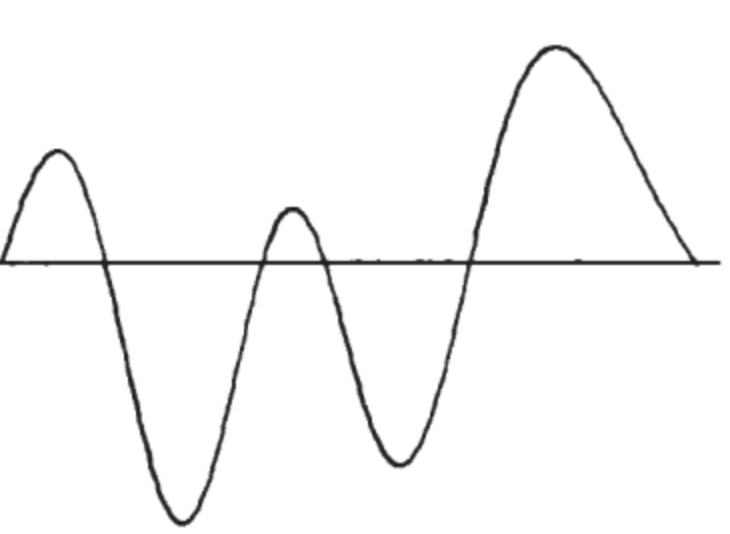
\includegraphics[scale=0.6]{img/SoundSignal.png}
		
			Рис 1.1 — Звуковой сигнал на входе АЦП
\end{center}

\begin{center}
		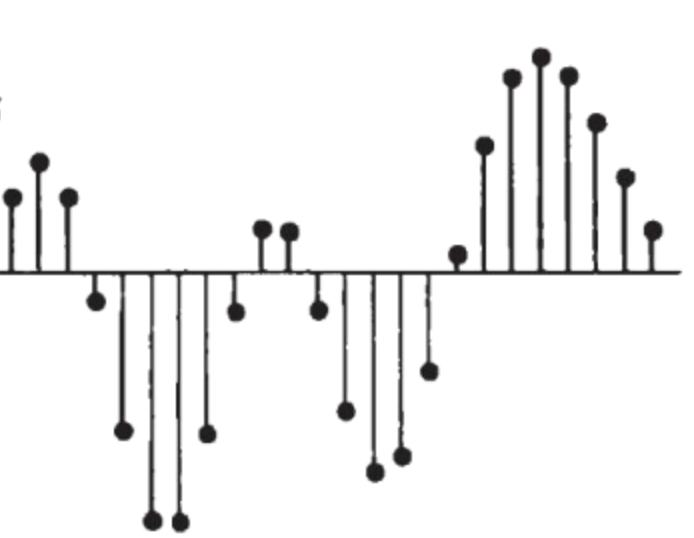
\includegraphics[scale=0.6]{img/DigitalSignal.png}
		
			Рис 1.2 — Дискретный сигнал на выходе АЦП
\end{center} 

Обратное преобразование для воспроизведения звука, закодированного числовым кодом, выполняют цифро-аналоговые преобразователи (ЦАП). 

На рисунках 1.3 и 1.4 представлено обратное преобразование дискретного сигнала в непрерывный звуковой сигнал.

\begin{center}
		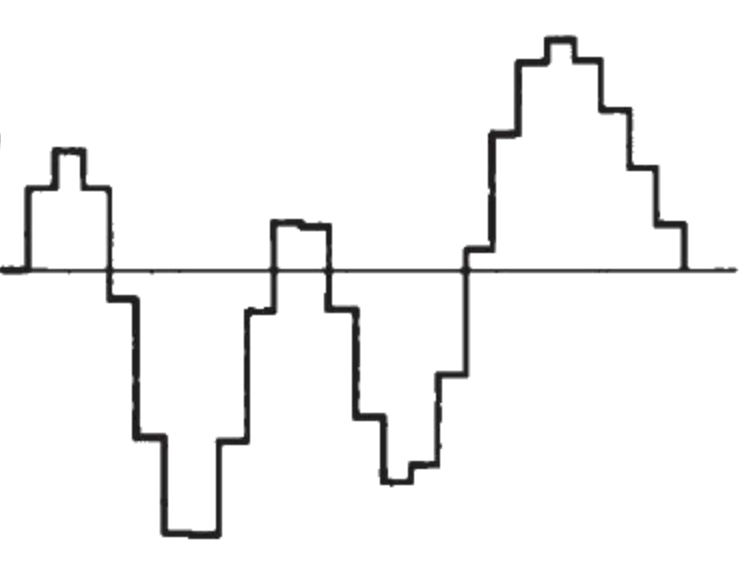
\includegraphics[scale=0.5]{img/DigitalSignal2.png}
		
			Рис 1.3 — Дискретный сигнал на входе ЦАП
\end{center} 

\newpage

\begin{center}
		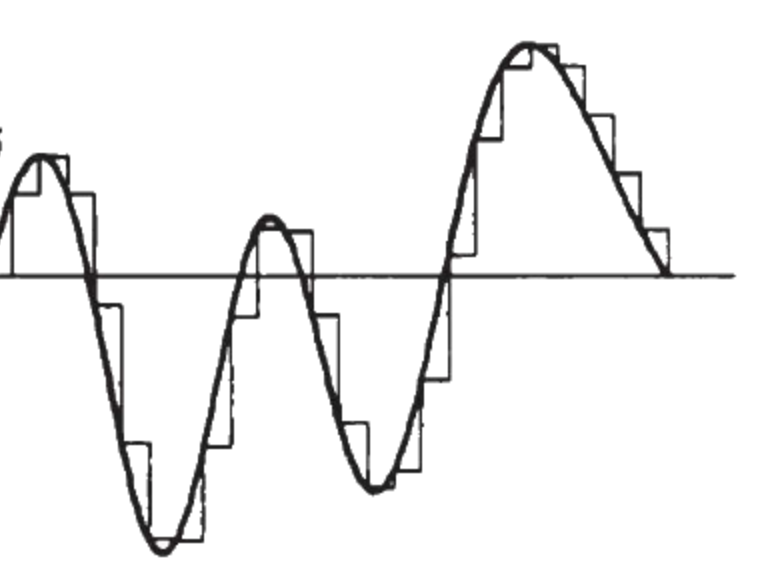
\includegraphics[scale=0.5]{img/SoundSignal2.png}
		
			Рис 1.4 — Звуковой сигнал на выходе ЦАП
\end{center} 

Недостатком данного метода кодирования является то, что синтезированные звуки получаются не слишком похожими на звучание реальных инструментов или других источников закодированного звука.

Таблично-волновой метод (Wave-Table) основан на том, что в заранее подготовленных таблицах хранятся образцы звуков окружающего мира, музыкальных инструментов и так далее. Числовые коды выражают высоту тона, продолжительность и интенсивность звука и прочие параметры, характеризующие особенности звука. Поскольку в качестве образцов используются «реальные» звуки, качество звука, полученного в результате синтеза, получается очень высоким и приближается к качеству звучания реальных музыкальных инструментов \cite{TypesofSynthesis}.

\subsection{Хранение аудиоинформации на компьютере}
Для хранения звуковых данных на компьютере и звуковых носителях в аудиофайлах используются цифровые аудиоформаты. При этом звуковые данные могут быть сжаты для устранения избыточности с помощью устройства или программы, называемой аудиокодеком. Выделяется три основных типа аудиоформатов:
\begin{itemize}
	\item[---]  аудиоформаты без сжатия;
	\item[---]  аудиоформаты со сжатием без потерь;
	\item[---]  аудиоформаты со сжатием с потерями.
\end{itemize}

Некоторые примеры аудиоформатов представлены в таблицах 1 --- 2 \cite{AudioFormats}.

\begin{table}[H]
\caption{Примеры аудиоформатов (часть 1)}
\begin{center}
\begin{tabular}{|p{0.3\linewidth}|p{0.3\linewidth}|p{0.3\linewidth}|}
		\hline
		Расширение & Тип & Описание \\ [0.5ex] 
 		\hline
		 .wav на Windows или .aiff на MAC & Без сжатия & Гибкий аудиоформат, разработанный для хранения любой комбинации частот дискретизации оригинальной звукозаписи. Аудиофайлы с таким форматом достигают большого размера\\
 		\hline MP3 & Сжатие с потерями & Самый популярный аудиоформат. Значительное уменьшение размера данных\linebreak достигается за счет потери качества воспроизведения на профессиональных звуковых системах\\
 		\hline
 		FLAK & Сжатие без потерь & Не нарушает целостность данных, при этом обладая относительной быстротой кодирования/декодирования, гибкостью и средней степенью сжатия\\
		\hline
\end{tabular}
\end{center}
\end{table}

\begin{table}[H]
\caption{Примеры аудиоформатов (часть 2)}
\begin{center}
\begin{tabular}{|p{0.3\linewidth}|p{0.3\linewidth}|p{0.3\linewidth}|}
		\hline
		Расширение & Тип & Описание \\ [0.5ex] 
 		\hline
		AAC & Cжатие с потерями & Преемник MP3 формата с более эффективной компрессией\\
		\hline
		WMA & Сжатие с потерями & Разработан под ОС Windows. Полностью поддерживается Windows, однако при низкой степени сжатия потока качество звука заметно снижается\\
		\hline
		TAK & Cжатие без потерь & При отсутствии потерь в качестве отличается высокой скоростью кодирования/декодирования и степенью сжатия\\
		\hline
		RAW & Без сжатия & Содержит необработанную информацию для обеспечения целостности данных. Не имеет четкой спецификации\\
		\hline
\end{tabular}
\end{center}
\end{table}	

\subsection{MIDI-файлы}

Отдельно от приведенной в таблицах 1.1 -- 1.2 классификации рассматриваются аудиоформаты, содержащие не только оцифрованный звук или не содержащие его вовсе, такие как \textbf{MIDI} формат \cite{AITMAWC}, хранящий наборы инструкций для воспроизведения звука. Аббревиатура MIDI расшифровывается как Musical Instrument Digital Interface (Цифровой интерфейс музыкальных инструментов). Этот формат представляет собой интерфейс музыкальных инструментов, с помощью которого можно кодировать нажатие клавиш, проигрываемые ноты, ссылки на инструменты, значения изменяемых параметров звука и другие данные. Такой способ представления данных позволяет синхронизировать звуковое воспроизведение с управлением различным оборудованием.
При этом последовательность инструкций, хранимая в MIDI-файле, только аппроксимирует нюансы исполнения, игнорируя, например, динамические изменения в продолжительности ноты.
Главной целью разработки такого формата является компактное представление, которое подходит для хранения на дисковом пространстве, но может быть неудобно для хранения в памяти для быстрого доступа \cite{SMFFS}.
Файлы MIDI содержат один или несколько потоков MIDI с информацией о времени для каждого события. Поддерживаются структуры песен и дорожек, информация о темпе и тактовом размере. Названия дорожек и другая описательная информация могут храниться вместе с MIDI-данными. MIDI формат поддерживает несколько дорожек.

MIDI-файлы строятся из фрагментов. Каждый фрагмент имеет 4-символьный тип и 32-битную длину, которая представляет собой количество байтов в фрагменте. Каждый фрагмент начинается с 4-символьного ASCII типа. За ним следует 32-битная длина, старший байт идет первым (например, длина, равная 6 байтам, сохраняется, как 00 00 00 06). Эта длина относится к количеству байтов данных, которые следуют далее: восемь байтов, отведенных для типа и длины, не включены. Таким образом, фрагмент длиной 6 байтов фактически займет 14 байтов дискового пространства.

MIDI-файлы состоят из фрагментов 2-х типов: фрагмент заголовка и фрагмент дорожки. При этом такой файл всегда начинается с фрагмента заголовка, за которым следует один или несколько фрагментов дорожек.

На рисунке 1.5 представлена концепция структуры файла MIDI \cite{SMFFS}.
\begin{center}
		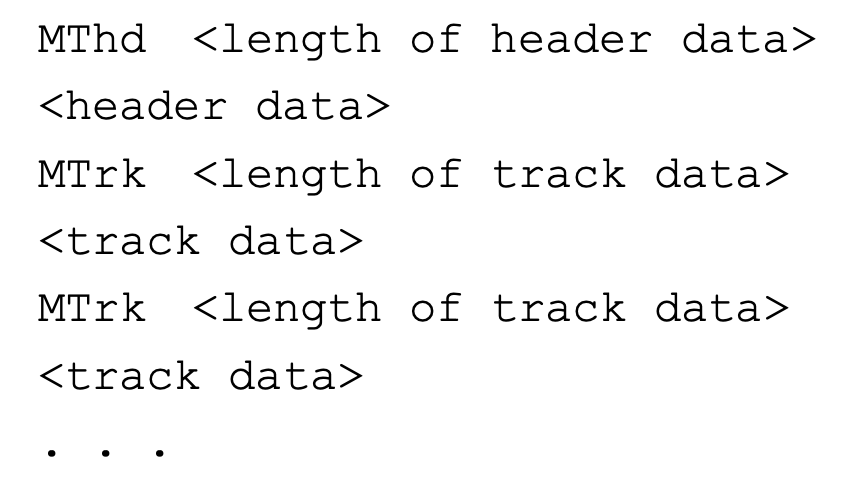
\includegraphics[scale=0.6]{tex/img/MidiStruct.png}
		
			Рис 1.5 — Общая структура файла MIDI
\end{center} 

Фрагмент заголовка предоставляет минимальный объем информации, относящейся ко всему MIDI-файлу и состоит из следующих элементов.
\begin{enumerate}
\item chunk type -- 4-х символьное представление типа фрагмента (MThd).
\item length -- 32-битная величина, значение которой описывает длину в байтах фрагмента без учета первых двух элементов (всегда 6).
\item format -- формат MIDI-файла (2 байта).
\begin{enumerate}
\item 0 -- файл содержит одну единственную дорожку, содержащую MIDI-данные, возможно, для всех 16 каналов. Используется, если секвенсор хранит все  MIDI-данные в одном блоке памяти в том порядке, в котором они воспроизводятся.
\item 1 -- файл содержит одну или несколько одновременных (то есть все начинаются с предполагаемого времени 0) дорожек, возможно, каждая на одном канале. Вместе эти треки считаются одной секвенцией или паттерном. Используется, если  секвенсор разделяет дорожки на разные блоки памяти, но воспроизводит их одновременно.
\item 2 -- файл содержит один или несколько последовательных независимых паттернов, состоящих из одной дорожки. Используется, если секвенсор разделяет дорожки на разные блоки памяти, но воспроизводит только один блок за раз (каждый блок считается отдельным «отрывком» или «песней»).
\end{enumerate}
\item ntrks -- количество дорожек.
\item division -- разрешение, указвающее, как MIDI-тики должны быть переведены во время.
\end{enumerate}

Фрагмент дорожки хранит саму музыкальную информацию и представляет собой поток MIDI-событий (и не MIDI-событий), которому предшествуют значения дельта-времени. 
Каждый такой фрагмент состоит из следуюших элементов.
\begin{enumerate}
\item chunk type -- 4-х символьное представление типа фрагмента (MTrk).
\item length -- 32-битная величина, значение которой описывает длину в байтах фрагмента без учета первых двух элементов.
\item MTrk event -- MIDI- или не MIDI-событие (может быть одно или несколько).
\end{enumerate}

В свою очередь, элемент MTrk event представляется следующими параметрами.
\begin{enumerate}
\item delta-time -- количество времени до следующего события (Если первое событие на дорожке происходит в самом начале дорожки, или если два события происходят одновременно, значение равно 0).
\item event -- либо MIDI-событие (например, такого содержания: идентификатор события, информация о воспроизводимой ноте, ее высоте и положении в октаве и сила извлечения звука), либо не MIDI-событие (события, которые содержат такие данные, как настройки темпа, названия дорожек и тому подобное).
\end{enumerate}

Благодаря такому формату, MIDI-файлы поддерживают хранение музыкальных партитур.
Музыкальная партитура \cite{P} -- это двухмерное представление звуковой последовательности, составляющей музыкальное произведение. Два основных параметра в таком представлении -- это музыкальные ноты, которые должен играть каждый инструмент, и момент, когда звучит каждая нота. Полнофункциональная партитура представляет другие параметры, потому что в партитуру помещается много других элементов, таких как интенсивность каждой ноты и ее изгиб. Тем не менее, два основных параметра достаточны для представления музыки. Таким образом, музыкальная партитура является инструкцией для воспроизведения звука и может храниться в MIDI аудиоформате. Причем в MIDI аудио-файле содержится только одна характеристика: последовательность нот, играемых каждым инструментом, — где ноты имеют начальное сообщение, указывающее на канал (1-16), номер высоты тона в полутонах (1-127), динамику (1-127) и сообщение, свидетельствующее об окончании ноты \cite{AITMAWC}.

Таким образом, MIDI-файлы могут содержать разнообразную информцию о музыке, не ограничиваясь только оцифрованным звуком. При этом формат MIDI разработан так, что даже подробная информация, включающая, например, метаданные и сложные инструкции для воспроизведения нот через различное музыкальное оборудование, имеет компактное представление. Учитывая эти достоинства, дальнейшее рассмотрение аудио-файлов в данной работе ограничивается MIDI форматом, для структуры которого разрабатывается метод распределенного хранения в NoSQL-базе данных.

\clearpage

\section{Существующие решения}

\subsection{Хранение MIDI-файлов в реляционной базе данных PostgreSQL в виде блоба}

\textbf{PostgreSQL} — свободная объектно-реляционная система управления базами данных \cite{PSQL}. 
PostgreSQL предоставляет средства работы с медиафайлами, рассматривающие такие файлы, как большие объекты, или, иначе говоря, блобы (специальный тип данных, предназначенный, в первую очередь, для хранения аудиофайлов и изображений, а также компилированного программного кода) \cite{BLOB}. Механизм больших объектов разбивает данные большого объема на «фрагменты» и сохраняет эти фрагменты в строках таблицы. При произвольном доступе на запись и чтение быстрый поиск нужного фрагмента обеспечивается индексом-B-деревом в этой таблице. Аудиофайлы, записанные в базу данных таким способом, представляются потоком байтов, разбитым на сегменты, каждый из которых не превышает величину LOBLKSIZE (2,05 Кб) для удобного размещения в отдельных строках таблицы \cite{DPSQL}. Потоковый доступ удобен в обработке данных больших объемов, которыми неудобно или невозможно оперировать как одним целым. К тому же это расширяет возможности доступа к отдельным частям данным, что обуславливается механизмом работы со структурой большого объекта: так как данные разбиты на фрагменты, каждый из которых представляет собой кортеж, можно легко получить доступ к любому такому фрагменту без необходимости считывать весь объект. Однако такой подход не позволяет извлечь конкретную часть данных, если не знать структуру хранимого объекта, а именно какой набор байт какой части данных соответствует. Это приводит к тому, что такой способ хранения не подойдет, в случае если необходимо не только хранить и извлекать аудиофайл из базы данных целиком, но и изменять отдельные его части.  

На рисунке 1.6 представлена концептуальня схема хранения MIDI-файлов в базе данных в виде блоба \cite{CBMS}.
\begin{center}
		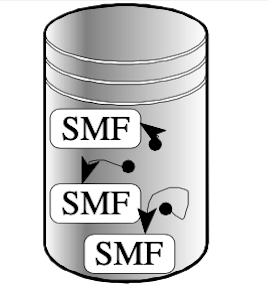
\includegraphics[scale=0.7]{img/blob}
		
			Рис 1.6 — Хранение MIDI-файлов в базе данных в виде блоба
\end{center} 

В PostgreSQL большие объекты хранятся в таблице pg\_largeobject, имеющей следующую структуру (таблица 1.3) \cite{PSQL}.

\begin{table}[H]
\caption{Структура таблицы pg\_largeobject}
\begin{center}
\begin{tabular}{|p{0.3\linewidth}|p{0.3\linewidth}|p{0.3\linewidth}|}
		\hline
		Имя & Тип & Описание \\ [0.5ex] 
 		\hline
		loid & oid & Идентификатор большого объекта, включающего эту страницу\\
		\hline
		pageno & int4 & Номер этой страницы в большом объекте (начиная с 0)\\
		\hline
		data & bytea & Данные, хранящиеся в большом объекте\\
		\hline
\end{tabular}
\end{center}
\end{table}

Для добавления в базу данных большого объекта, сформированного из аудио-файла, существует серверная функция lo\_import(), принимающая путь к файлу на диске. Возвращаемым значением этой функции является идентификатор созданного большого объекта (тип данных oid). Пример добавления содержимого аудио-файла в базу данных PostgreSQL при наличии созданной заранее таблицы audio c атрибутом bigObject\_Id типа oid представлен на листинге \ref{lst:lo_import}.

\newpage

\begin{lstlisting}[language=sql, label=some-code, caption=Пример добавления аудио-файла в базу данных PostgreSQL в виде блоба, label=lst:lo_import]
INSERT INTO audio (bigObjectId)
    VALUES (lo_import("/Users/anastasia/Desktop/ProgramEngineering/audio.mid"));
\end{lstlisting}

В результате, считанные из файла байты, будут добавлены в таблицу pg\_largeobject в виде фрагментов большого объекта. Однако, при таком способе хранения аудио-файла для систем управления базами данных (СУБД) он представляется, как аморфный набор данных, так как СУБД не знает внутренней структуры блоба. Таким образом, операции доступа к конкретным данным MIDI-файла оказываются невозможны.

\subsection{Хранение путей к MIDI-файлу в файловой системе}

Одним из возможных решений хранения аудио-файла в любой базе данных является хранение в базе данных пути к файлу на диске.

На рисунке 1.7 представлена концептуальня схема хранения аудио-файлов в базе данных с использованием пути к файлу \cite{CBMS}.
\begin{center}
		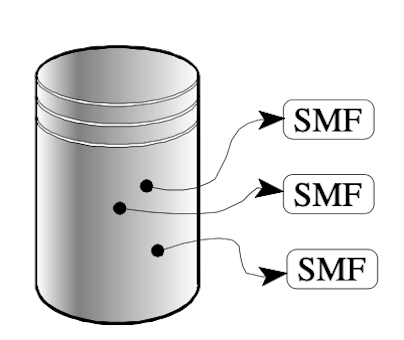
\includegraphics[scale=0.7]{img/disk}
		
			Рис 1.7 — Хранение в базе данных путей к MIDI-файлам, расположенным на дисковом пространстве
\end{center} 

Данный подход не выгоден, так как ответственность за хранилище и расположение файлов в нем полностью делегируется на операционную систему, из-за чего СУБД не может гарантировать целостность набора указателей, а также вся дальнейшая работа с MIDI-файлом предоставляется клиенту, что значительно снижает роль базы данных при таком методе хранения. 

\subsection{Хранение MIDI-файла в виде структуры}

Спецификация MIDI-файлов \cite{SMFFS} позволяет определить внутреннюю структуру аудио-файла, в которой его можно было бы хранить в базе данных. Такой подход удовлетворяет требованию распределенности и возлагает значительную степень ответственности за работу с аудио-информацией на базу данных, освобождая клиента от необходимости использовать дополнительные инструменты, в случае если задача заключается в доступе к определенным элементам структуры MIDI-файла. 

На рисунке 1.8 представлена концептуальня схема хранения аудио-файлов в базе данных на основе их структуры \cite{CBMS}.
\begin{center}
		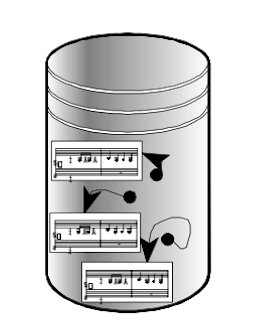
\includegraphics[scale=0.7]{img/musical_scores}
		
			Рис 1.8 — Хранение MIDI-файлов в базе данных на основе их структуры
\end{center} 

Предварительный анализ исходного MIDI-файла в том виде, в котором он хранится на диске, позволит СУБД впоследствии работать со структурированными данными MIDI-файла и, соответственно, отвечать на запросы на основе содержимого хранимой информации, что является наиболее выгодным решением.

\section{Виды существующих NoSQL баз данных}
 \textbf{NoSQL} база данных \cite{WNOSQL} — это база данных, которая не использует реляционную модель данных, а именно организацию хранения данных в виде таблиц и отношений между ними. Вместо этого такие базы ориентированы на какой-то определенный тип данных, под требования хранения которого оптимизируется система хранения таким образом, чтобы процесс запроса был наиболее подходящим для выбранного типа данных. Это позволяет хранить любые данные в NoSQL базах нерегламентированно (гибкость модели данных), а также размещать данные большого объема с относительно быстрым доступом к ним за счет масштабируемости. Главное правило проектирования структуры данных в NoSQL базах — она должна подчиняться требованиям приложения и быть максимально оптимизированной под наиболее частые запросы. Термин "NoSQL" расшифровывается как "Not Only SQL" и, подразумевая под собой ответвление SQL-подхода к проектированию баз данных, является собирательным определением альтернатив к организации хранения и доступа к данным средствами SQL. 
 
 По модели данных NoSQL-базы данных классифицируются на следующие основные виды.
\begin{enumerate}
\item Ключ — значение.
\item Документы.
\item Семейства столбцов.
\item Графы.
\end{enumerate}

 В таблицах 1.4 --- 1.6 представлена сравнительная характеристика баз данных SQL и NoSQL \cite{AMNOSQL}.

\clearpage 

\begin{table}[h]
\caption{Сравнительная характеристика баз данных SQL и NoSQL (часть 1)}
\begin{center}
\begin{tabular}{|l|p{0.25\linewidth}|p{0.41\linewidth}|p{0.35\linewidth}|}
		\hline
		Критерий/Тип БД & Реляционные & NoSQL \\ [0.5ex] 
 		\hline
		 Модель данных & Используют реляционную модель, которая преобразует данные в двумерные таблицы, состоящие из строк и столбцов & Используют разнообразные модели данных, такие как пары «ключ-значение», документы и графы, оптимизированные под определенный тип хранимых даных для высокой производительности и горизонтальной масштабируемости\\
 		\hline 
		Схема данных & Схема жестко задает таблицы, строки, столбцы, индексы, отношения между таблицами и прочие элементы базы данных. Такая БД обеспечивает целостность ссылочных данных в отношениях между таблицами. & Гибкая схема\\
 		\hline
 \end{tabular}
\end{center}
\end{table}

\clearpage

\begin{table}[h]
\caption{Сравнительная характеристика баз данных SQL и NoSQL (часть 2)}
\begin{center}
\begin{tabular}{|l|p{0.25\linewidth}|p{0.41\linewidth}|p{0.35\linewidth}|}
		\hline
		Критерий/Тип БД & Реляционные & NoSQL \\ [0.5ex] 
		\hline
		Выполнение запросов & Запросы составляются на языке SQL. Эти запросы анализирует и выполняет реляционная база данных & Для записи/извлечения могут использоваться объектно-ориентированные API. Поиск может осуществляться по парам «ключ-значение», наборам столбцов и т. д.\\
		\hline
		Масштабирование & Обычно масштабируются путем увеличения вычислительных возможностей аппаратного обеспечения или добавления отдельных копий для рабочих нагрузок чтения (преимущественно вертикальное масштабирование) & Обычно поддерживают высокую разделяемость благодаря шаблонам доступа с возможностью масштабирования на основе распределенной архитектуры. Это повышает пропускную способность и обеспечивает устойчивую производительность почти в неограниченных масштабах (горизонтальное масштабирование)\\
		\hline
\end{tabular}
\end{center}
\end{table}

\clearpage

\begin{table}[h]
\caption{Сравнительная характеристика баз данных SQL и NoSQL (часть 3)}
\begin{center}
\begin{tabular}{|l|p{0.25\linewidth}|p{0.41\linewidth}|p{0.35\linewidth}|}
		\hline
		Критерий/Тип БД & Реляционные & NoSQL \\ [0.5ex] 
 		\hline
 		Производительность & Производительность главным образом зависит от дисковой подсистемы. Для обеспечения максимальной производительности часто требуется оптимизация запросов, индексов и структуры таблицы. & Производительность обычно зависит от размера кластера базового аппаратного обеспечения, задержки сети и вызывающего приложения\\
 		\hline
\end{tabular}
\end{center}
\end{table}

\clearpage

\subsection{Модель данных Ключ-Значение}

Модель данных, реализующяя хранение по типу ключ‑значение связывает каждое значение данных с уникальным ключом. Большинство СУБД с такой моделью данных поддерживают только самые простые операции запроса, вставки и удаления, а также, как правило, используют хеш-таблицу, в которой находится уникальный ключ и указатель на конкретный объект данных. Производительность сильно вырастает за счёт кеширующих механизмов. 
Как ключи, так и значения могут представлять собой что угодно: от простых до сложных составных объектов. Базы данных с использованием пар ключ‑значение поддерживают высокую разделяемость и обеспечивают беспрецедентное горизонтальное масштабирование, недостижимое при использовании других типов баз данных. Однако, чтобы частично или полностью изменить значение, приложение всегда перезаписывает существующее значение целиком. Также СУБД, имеющие такую модель данных, не оптимизированы для запросов по значению.

\subsection{Модель данных документов}

Документоориентированная модель данных хранит данные, представленные парами ключ-значение, которые сжимаются в виде полуструктурированного документа из тегированных элементов, подобно JSON, XML, BSON и другим подобным форматам. В базе данных документов хранится коллекция документов, в которой каждый документ состоит из именованных полей и данных. Данные могут быть простыми значениями или сложными элементами, такими как списки и дочерние коллекции. Документы извлекаются по уникальным ключам. 

Одним из ключевых различий между моделью данных по типу ключ-значение и документоориентированным хранением является то, что последнее включает метаданные, связанные с хранимым содержимым, что даёт возможность делать запросы на основе содержимого. Тот факт, что такие базы данных работают без схемы, делает простой задачей добавление полей в документы без необходимости сначала заявлять об изменениях. 

Документные базы данных позволяют разработчикам хранить и запрашивать данные в БД с помощью той же документной модели, которую они используют в коде приложения. Гибкий, полуструктурированный, иерархический характер документов и документных баз данных позволяет им развиваться в соответствии с потребностями приложений.Документные базы данных обеспечивают гибкость индексации, производительность выполнения стандартных запросов и аналитику наборов документов.

\subsection{Модель данных семейства столбцов}

В колоночных NoSQL-базах данных данные хранятся в ячейках, сгруппированных в колонки, а не в строки данных. Колонки логически группируются в колоночные семейства. Колоночные семейства могут состоять из практически неограниченного количества колонок, которые могут создаваться во время работы программы или во время определения схемы. Чтение и запись происходит с использованием колонок, а не строк.

В сравнении с хранением данных в строках, как в большинстве реляционных баз данных, преимущества хранения в колонках заключаются в быстром поиске/доступе и агрегации данных. Реляционные базы данных хранят каждую строку как непрерывную запись на диске. Разные строки хранятся в разных местах на диске, в то время как колоночные базы данных хранят все ячейки, относящиеся к колонке, как непрерывную запись, что делает операции поиска/доступа быстрее.

В отличие от модели данных на основе пар ключ-значение и модели данных документов, большинство хранилищ столбцов используют для упорядоченного хранения данных сами значения ключей, а не хеш-коды от них. Многие реализации позволяют создавать индексы по определенным столбцам в семействе столбцов. Индексы позволяют получать данные по значениям столбцов, а не ключам строки. 

\subsection{Модель данных графов}

В графовой базе данных нет строгого формата SQL или представления таблиц и колонок, вместо этого используется гибкое графическое представление, которое подходит для решения проблем масштабируемости. База данных графов хранит сведения двух типов: узлы и грани. Ребра задают связи между узлами. Узлы и ребра могут иметь свойства, предоставляющие сведения об этом узле или ребра, аналогичные столбцам в таблице. Грани могут иметь направление, указывающее на характер связи. Обход графа в графовой базе данных можно выполнять либо по определенным типам ребер, либо по всему графу. Обход соединений или взаимосвязей в графовых базах данных выполняется очень быстро, поскольку взаимосвязи между узлами не вычисляются во время выполнения запроса, а хранятся в базе данных. Тем не менее, модель данных графов отличается высокой сложностью реализации.

\subsection{MongoDB}

MongoDB  \cite{Mongo} -- система управления базами данных, которая работает с документоориентированной моделью данных и для хранения данных использует формат, подобный JSON \cite{JSON}, -- формат BSON \cite{BSON}. Данный формат представляет собой двоично-кодированную сериализацию JSON-подобных документов. Как и JSON, BSON поддерживает встраивание документов и массивов в другие документы и массивы. BSON также содержит расширения, позволяющие представлять типы данных, не входящие в спецификацию JSON. Например, BSON имеет тип BinData \cite{BinData}.

Данные в BSON-формате хранятся в документах, которые хранятся в коллекции. Это означает, что структура сохраняемых данных может быть изменена для каждой записи и не требуется, чтобы она соответствовала предварительно определенному шаблону. Хранилище в BSON-формате также позволяет вкладывать данные, благодаря чему можно хранить сложноорганизованные данные с любой структурой. MongoDB поддерживает поиск по полям, диапазонные запросы и поиск по регулярным выражениям. Могут быть сделаны запросы для возврата определенных полей в документах. Также MongoDB использует концепцию шардинга для горизонтального масштабирования с помощью разделения данных между несколькими экземплярами БД. Она может работать на нескольких серверах, балансируя нагрузку и/или дублируя данные, чтобы поддерживать работоспособность системы в случае аппаратного сбоя. 

Терминология MongoDB отличается от терминологии SQL. Основные понятия баз данных сопоставлены в таблице 1.7.

\begin{table}[H]
\caption{Сравнение терминологии MongoDB и терминологии SQL}
\begin{center}
\begin{tabular}{|p{0.3\linewidth}|p{0.3\linewidth}|}
		\hline
		MongoDB & SQL \\ [0.5ex] 
 		\hline
		Коллекция & Таблица \\
		\hline
		Документ & Ряд \\
		\hline
		Поле & Столбец \\
		\hline
		ObjectId & Первичный ключ \\
		\hline
\end{tabular}
\end{center}
\end{table}

\section{Выбор NoSQL-базы данных}

В качестве NoSQL-базы данных, наиболее подходящей под хранение аудио-файлов формата MIDI на основе их структуры, была выбрана база данных MongoDB, так как она является свободной и одной из самых распространенных документоориентированных баз данных. Это означает, что структура сохраняемых данных может быть изменена для каждой записи в базу и не требует, чтобы она была в предварительно определенном формате. Хранилище в формате BSON, отличающемся гибкой структурой, высокой скоростью сканирования и кодирования и декодирования данных, а также наличием типов данных, не поддерживаемых форматом JSON, позволяет вкладывать данные, что особенно важно для хранения аудио-файлов в MIDI формате, содержащих произвольное количество музыкальных дорожек. Возможность хранения разных типов данных в непредопределенной стрктуре позволяет хранить музыкальные данные в любом формате, адаптируемом под бизнес-требования. В частности, такой тип, как "бинарные данные" (BinData), очень удобен для представления некоторых элементов MIDI-файлов, например, для массива байтов, отвечающих за MIDI- и не Midi-события во фрагменте музыкальной дорожки. Помимо этого, MongoDB предоставляет возможности репликации и ограниченную поддержку шардинга, что обеспечивает высокие доступность и надежность и балансировку нагрузки. Также у MongoDB есть клиентские библиотеки для основных языков программирования, таких как C \cite{C}, C++ \cite{CPP}, C\# \cite{CS}, Python \cite{Python}, Java \cite{Java} и других. Открытый исходный код предоставляет возможность изучить внутреннее устройство СУБД и разработать программное обеспечение, которое впоследствии может быть интегрировано в систему.

\subsection{Выводы из аналитического раздела}

В данном разделе были приведены теоретические сведения о звуковой информации, об аудио-форматах и о существующих NoSQL-базах данных, а также были рассмотрены способы хранения аудио-файлов в базе данных. Было выяснено, что наиболее полноценную и разнородную информацию содержат аудио-файлы формата MIDI, которые наиболее оптимально хранить на основе их внутренней структуры. Также была приведена сравнительная характеристика реляционных и NoSQL-баз данных и сравнительная характеристика видов нереляционных баз данных по модели данных. На основе полученного сравнительного анализа, было установлено, что наиболее подходящим решением для хранения MIDI-файлов на основе их структуры является хранение в документоориентированной NoSQL-базе данных MongoDB.

\clearpage


%%% Local Variables:
%%% mode: latex
%%% TeX-master: "rpz"
%%% End:
